

\section{Making on-sky Sources%
  \label{making-on-sky-sources}%
}

On-sky target source objects for ScopeSim can be created in two ways:
by using the helper functions provided in the \href{https://scopesim-templates.readthedocs.io/en/latest/}{ScopeSim\_Templates} package, or by creating a \texttt{Source} object from scratch.
The latter requires the user to have both the spatial and spectral data needed to describe the object.


\subsection{ScopeSim Templates%
  \label{scopesim-templates}%
}

A useful addition to the ScopeSim eco-system is the package \texttt{ScopeSim\_templates}.
This python package provides so-called helper functions for generating ScopeSim readable \texttt{Source} object for common astronomical objects.
The \texttt{basic} subpackage contains functions for generating star clusters and grids of stars, as well as analytical and numerical representations of galaxies.
The documentation for \href{https://scopesim-templates.readthedocs.io/en/latest/}{ScopeSim templates can be found on Read-The-Docs}.

Here is a basic example of creating a star cluster using \texttt{ScopeSim\_templates}:

\phantomsection\label{code-scopesim-templates-example}
\begin{DUclass}{code}
\begin{DUclass}{plot}
\begin{quote}
\begin{alltt}
\begin{lstlisting}[frame=single]
from scopesim_templates.basic.stars import cluster

my_cluster = cluster(mass=1000, distance=50000,
                     half_light_radius=1)
\end{lstlisting}
\end{alltt}
\end{quote}
\end{DUclass}
\end{DUclass}

% action: plot
% name: scopesim_templates_cluster_example
% ---
% plt.figure(figsize=(10,10))
% my_cluster.plot()
% plt.xlabel("x [arcsec]")
% plt.ylabel("y [arcsec]")

% \begin{figure}[H]
% \noindent\makebox[\linewidth][c]{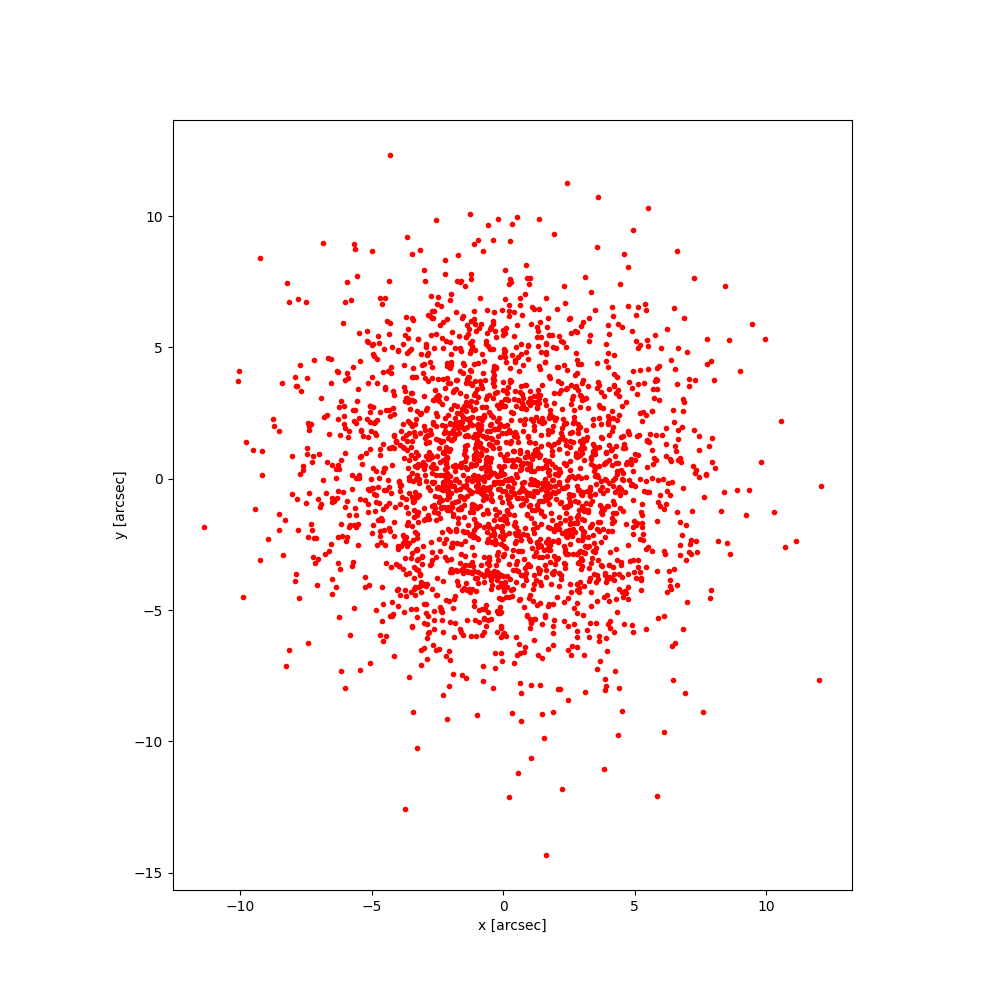
\includegraphics[scale=0.500000]{images/scopesim_templates_cluster_example.png}}\phantomsection\label{fig-scopesim-templates-cluster-example}
% \end{figure}

In section 7, various helper functions are used to create the source objects observed in the presented use cases.


\subsection{The ScopeSim Source object%
  \label{the-scopesim-source-object}%
}

The \texttt{Source} object is the underlying python class that contains the spatial and spectral descriptions of the on-sky target.
The spatial description can be either a table of point source positions, or a 2D intensity map (image) of an extended object.

Point source tables must contain the following columns:

\setlength{\DUtablewidth}{\linewidth}
\begin{longtable*}[c]{|p{0.107\DUtablewidth}|p{0.833\DUtablewidth}|}
\hline
\textbf{%
Column
} & \textbf{%
Description
} \\
\hline
\endfirsthead
\hline
\textbf{%
Column
} & \textbf{%
Description
} \\
\hline
\endhead
\multicolumn{2}{c}{\hfill ... continued on next page} \\
\endfoot
\endlastfoot

x, y
 & 
{[}arcsec{]} position of source relative to centre of FOV
\\
\hline

ref
 & 
index of spectrum associated with the point source
 \\
\hline

(weight)
 & 
{[}default=1{]} scaling factor if multiple point sources reference the same spectrum
 \\
\hline
\end{longtable*}

Extended objects intensity maps (images) must be \texttt{astropy.fits.HDUImage} objects that display a the extent of similar spectral regions.
Each image may only be linked to one spectrum.
An extended \texttt{Source} may however contain multiple images that reference different spectra.
To illustrate the point, a spiral galaxy may be split into two intensity maps (images).
The first shows the distribution of the new stellar population, while the second shows the distribution of the old stellar population.
Each of these images is linked to a generic spectrum for the given population.
Conceivably a third image showing the distribution of warm gas and the spectrum for warm gas could be added to the \texttt{Source} object.

Each ImageHDU must contain the following information in the header:

\setlength{\DUtablewidth}{\linewidth}
\begin{longtable*}[c]{|p{0.179\DUtablewidth}|p{0.412\DUtablewidth}|}
\hline
\textbf{%
Header Keyword
} & \textbf{%
Description
} \\
\hline
\endfirsthead
\hline
\textbf{%
Header Keyword
} & \textbf{%
Description
} \\
\hline
\endhead
\multicolumn{2}{c}{\hfill ... continued on next page} \\
\endfoot
\endlastfoot

CDELT1, CDELT2
 & 
Pixel scale of the image
 \\
\hline

CUNIT1, CUNIT2
 & 
Unit of the pixel scale value.
 \\
\hline

SPEC\_REF
 & 
Spectrum associated with the image
 \\
\hline
\end{longtable*}

All \texttt{Source} objects require list of one or more spectra to be passed to the \texttt{Source} object when it is created.
Spectra can either be \texttt{synphot.SourceSpectrum} objects or numpy arrays.
If they are passed as numpy arrays, a corresponding wavelength array must also be passed.

\DUadmonition[note]{
\DUtitle[note]{Note}

The ScopeSim affiliate packages \texttt{Spextra} and \texttt{Pyckles} provide access to many standard spectral libraries.

These python packages return spectra in a variety of formats including the \texttt{synphot.SourceSpectrum} format.
}

The following code shows the process of creating a simple binary star system from scratch:

\begin{quote}
\begin{alltt}
\begin{lstlisting}[frame=single]
# Get two spectra
from pyckles import SpectralLibrary
pickles = SpectralLibrary("pickles", return_style="synphot")
spec = [pickles.A0V, pickles.G2V]

# Make a table
from astropy.table import Table
tbl = Table(names=["x", "y", "ref"],
            data=[[-2, 2], [0, 0], [0, 1]])

# Combine spectra and positions in the Source object
from scopesim import Source
binary = Source(table=tbl, spectra=spec)
\end{lstlisting}
\end{alltt}
\end{quote}

Source objects can also be combined using the \texttt{+} operator:

\begin{quote}
\begin{alltt}
\begin{lstlisting}[frame=single]
star = Source(x=[0], y=[10], ref=[0], spectra=[pickles.M0III])
trinary = binary + star
\end{lstlisting}
\end{alltt}
\end{quote}

The \texttt{trinary} Source object now contains two tables with the positions of the stars and three spectra.
This can be verified by looking at the \texttt{<Source>.fields} and \texttt{<Source>.spectra} attributes.

We can also combine point source with extended source objects.
Each object remains intact inside the new \texttt{Source} container.

% Contents
% - What is inside a Source object
% - How to make source objects to observe
%     - Star cluster
%     - Custom point source
%     - Elliptical galaxy
%     - Custom extended source
%     - Combining sources
